\documentclass[journal]{vgtc}

\onlineid{0}
\vgtccategory{Research}

% ^^
\title{Pseudocode-Map Substitution Grows with Expertise: An Eye-Tracking Study}
% ^^

\author{%
  \authororcid{Razieh Fathi}{0000-0000-0000-0000},
  \authororcid{[SECOND AUTHOR]}{0000-0000-0000-0000},
  and
  \authororcid{Ian Handy}{0000-0000-0000-0000}
}

\authorfooter{
  \item
    Razieh Fathi is with [INSTITUTION].
    E-mail: [EMAIL]
  \item
    [SECOND AUTHOR] is with [INSTITUTION].
    E-mail: [EMAIL]
  \item
    Ian Handy is with [INSTITUTION].
    E-mail: [EMAIL]
}

% ^^
\abstract{%
  We tracked 62 participants' gaze across three programming expertise
  levels as they watched BFS and DFS algorithm animations with a
  pseudocode panel and a geospatial map, using a Tobii eye-tracker at
  60~Hz. Each participant viewed both algorithms, yielding 117
  analyzable trials. At the participant level, the Spearman correlation
  between pseudocode and map total fixation duration grows more
  negative as expertise increases: G1 shows no relationship
  ($r$=$-$0.03, ns), G2 a moderate negative correlation
  ($r$=$-$0.46, $p$=.04), and G3 a strong one ($r$=$-$0.63, $p$=.003),
  with the G1 vs G3 contrast significant under Fisher z ($p$=.04).
  Pseudocode and map dwell times trade off more strongly as
  programming expertise grows, consistent with the Expertise Reversal
  Effect. A directional sign reversal in fixation count correlation
  points the same way but does not reach significance. Split-panel
  designs validated at one expertise level may not generalize to
  others.
}
% ^^

\keywords{eye-tracking, algorithm visualization, expertise reversal effect, dual representation, representation substitution}

\graphicspath{{figs/}{figures/}{pictures/}{images/}{./}}

\usepackage{booktabs}
\usepackage{mathptmx}

\begin{document}

\firstsection{Introduction}

\maketitle

Previous studies have suggested that multi-channel communication leads to
higher learning outcomes~\cite{Mayer2001Multimedia}. Split-panel algorithm
visualizations are built on this assumption: the pseudocode lists each step and
the animated graph shows those steps running on a graph.

The multi-channel approach seems to affect engagement non-linearly in relation
to previous experience. Our study extends upon the Expertise Reversal Effect
and Cognitive Load Theory~\cite{Kalyuga2003Expertise,Sweller1988Cognitive}
and could help indicate the conditions under which these approaches are most
suitable. Prior work has not asked which viewers integrate both panels and
which do not.
% ^^
We ask whether dual-panel engagement is uniform across expertise levels or
whether attention on the two panels shifts from independence toward
substitution as prior knowledge grows.
% ^^

There have been numerous prior eye-tracking studies on algorithm comprehension,
but the focus of such studies is usually on transition counts or fixation
timing, not the directionality of the relationship between the two panels.
% ^^
Our study uses Spearman correlation between dwell times on the two AOIs as
the unit of measurement. Correlation is what a substitution pattern requires;
transition counts cannot show whether time on one panel trades off against
time on the other.

Our contributions are: (1)~to our knowledge, the first participant-level
evidence that pseudocode-panel and geospatial-map dwell times trade off
more strongly as programming expertise increases, (2)~a correlation-based
operationalization of this representation substitution, and (3)~design
implications for algorithm visualizations targeted at specific expertise
levels.
% ^^


\section{Related Work}

Mayer's CTML holds that learning improves when verbal and pictorial information
are processed through separate cognitive channels and integrated in working
memory~\cite{Mayer2001Multimedia}. Split-panel algorithm visualizations apply
this idea directly.

Working memory capacity is limited. Sweller's Cognitive Load Theory predicts
that a second representation increases cognitive load, and if intrinsic load
is already high, that addition hurts more than it
helps~\cite{Sweller1988Cognitive,Sweller1994Cognitive}. Viewers with no prior
knowledge of BFS or DFS face a novel algorithm and a novel visual format at
the same time.

The Expertise Reversal Effect predicts that as learners gain knowledge,
instructional supports that were once useful become redundant or
harmful~\cite{Kalyuga2003Expertise}. A viewer building a schema for BFS
benefits from pseudocode that labels each step. A viewer who already knows BFS
does not need that label.

% ^^
Both theories predict a monotonic decline in pseudocode dependence from G1
to G3. Neither explicitly predicts how dwell time on pseudocode and map
should trade off within a single viewer; we test that prediction directly.
Gegenfurtner et~al.'s meta-analysis of 296 eye-tracking studies found that
intermediate learners show longer fixation durations than both novices and
experts, a pattern that the novice-to-expert framing does not
predict~\cite{Gegenfurtner2011Expertise}.
% ^^

Bednarik studied attentional strategies during debugging with multiple code
representations and found that experts and novices behave
differently~\cite{Bednarik2012Expertise}. Experts consult secondary
representations to confirm a mental model they already hold; novices switch
between panels without a governing strategy. Our study adds the intermediate
group Bednarik did not include.

Richter and Scheiter measured process-level eye-tracking across text and
picture AOIs in multimedia learning tasks at two expertise
levels~\cite{Richter2019Studying}. Low-prior-knowledge learners coordinated
both AOIs when signaling cues were present; high-prior-knowledge learners did
not benefit. The setup is structurally similar to pseudocode and map AOIs in
our study.
% ^^
Neither Bednarik nor Richter and Scheiter included three expertise groups or
used correlation structure between dwell times as the measurement unit.
Detecting a substitution gradient requires both.
% ^^


\section{Study Design}

\subsection{Participants and Design}

Our study included 62 participants who watched animated algorithm
visualizations while wearing a Tobii eye-tracker recording at 60~Hz.
Participants were divided into three experience groups: G1 (no programming
experience), G2 (brief programming knowledge), and G3 (multiple years of
formal coursework). Each participant viewed both a BFS visualization and a
DFS visualization, yielding 117 analyzable trials ($n$=59 BFS, $n$=58 DFS)
after quality screening. The visualization style was Metal throughout, a
high-contrast, stylized rendering. Expertise group assignment was based on
self-reported programming background~[CONFIRM MEASUREMENT METHOD].

This study was conducted under the oversight of [INSTITUTION] IRB
(No.~[NUMBER]). Informed consent was obtained from all participants.

\subsection{Stimuli}

Each trial displayed a split-screen animation with a pseudocode panel on the
left and a geospatial map on the right. The geospatial map showed a graph of
nodes and edges where nodes activated as the algorithm visited them. Both
panels were visible simultaneously throughout the trial.

\subsection{Eye-Tracking Metrics}

Two Areas of Interest (AOIs) were defined: Pseudocode (left panel) and
Geospatial Map (right panel). The primary metrics were Fixation Count~(FC),
the number of individual fixation events per AOI, and Total Fixation
Duration~(TFD), total dwell time in seconds. Derived composite metrics
included the pseudocode-to-map ratio ($\text{TFD}_\text{pseudo} /
\text{TFD}_\text{map}$), scanner index ($\text{VC}_\text{pseudo} /
\text{TFD}_\text{pseudo}$), average fixation depth ($\text{TFD}_\text{pseudo}
/ \text{FC}_\text{pseudo}$), and switching rate
($(\text{VC}_\text{pseudo} + \text{VC}_\text{map}) /
(\text{TFD}_\text{pseudo} + \text{TFD}_\text{map})$).

\subsection{Statistical Methods}

Non-parametric methods were used throughout because eye-tracking metrics are
typically skewed and our group sizes are modest. Group comparisons used
Kruskal-Wallis with pairwise Mann-Whitney U post-hoc tests. Within-group
associations were measured using Spearman rank correlation. Group moderation
of correlation structure was tested via Fisher z-transformation, which
evaluates whether the Spearman $r$ between two metrics differs significantly
between groups. Partial Spearman correlation controlled for group and
algorithm condition.


\section{Results}

\subsection{Non-Monotonic Pseudocode Engagement}
\label{sec:inverted}

Our study suggests that participants who had some prior exposure to the subject
matter (G2) were likely to engage with the pseudocode panel notably longer than
either G1 or G3. The median pseudocode-to-map ratio was 9.57 for G1, 12.33
for G2, and 6.12 for G3. The inverted-U pattern holds across TFD and average
fixation depth.

The difference in pseudocode-to-map ratio between BFS and DFS conditions is
statistically significant in G1 ($p$=.040, $r$=0.43) and absent in both G2
and G3, suggesting that prior knowledge overrides the visual structure of the
algorithm.

% ^^
\subsection{Monotonic Substitution with Expertise}
\label{sec:reversal}

At the participant level (averaging each participant's BFS and DFS trials),
the Spearman correlation between pseudocode and map total fixation duration
grows more negative with expertise. G1 shows no relationship ($r$=$-$0.03,
ns, $n$=19), G2 a moderate negative correlation ($r$=$-$0.46, $p$=.04,
$n$=21), and G3 a strong negative correlation ($r$=$-$0.63, $p$=.003,
$n$=20). Pairwise Fisher z testing supports group moderation for the
endpoint contrast (G1 vs G3 $p$=.04); adjacent contrasts (G1 vs G2 $p$=.18,
G2 vs G3 $p$=.47) do not reach significance on their own. Participants who
dwell longer on one panel dwell proportionally less on the other, and this
trade-off grows steeper with programming expertise.

The same analysis using fixation count is directionally compatible but
weaker. FC correlation is flat in G1 ($r$=+0.04, $p$=.86), positive in G2
($r$=+0.33, $p$=.14), and negative in G3 ($r$=$-$0.16, $p$=.49);
\Cref{fig:core} shows the per-participant FC scatter. Pairwise Fisher z
tests on FC do not reach significance (G2 vs G3 $p$=.13; G1 vs G3 $p$=.55;
G1 vs G2 $p$=.38), so the sign reversal in visit counts is directional
rather than inferential at the participant level. The count of discrete
visits appears less sensitive to expertise than dwell time itself.
% ^^

\begin{figure*}[tb]
  \centering
  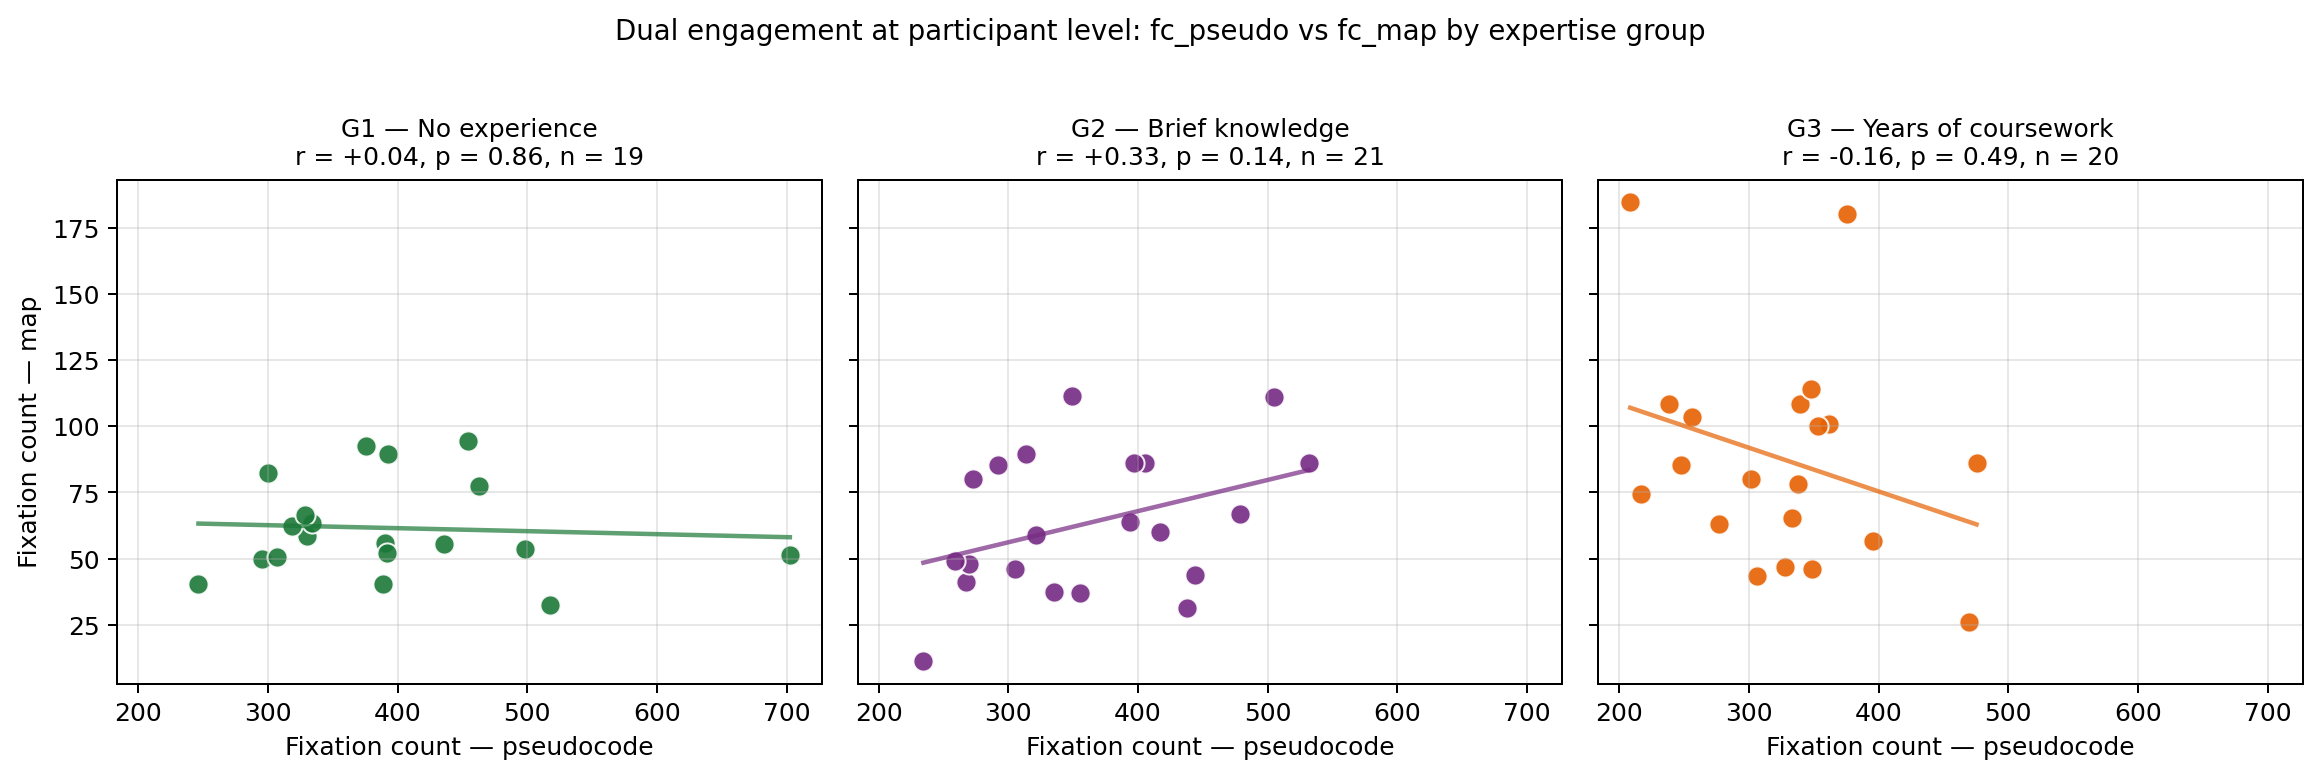
\includegraphics[width=\linewidth, alt={Scatter plot showing fixation count correlation between pseudocode and map AOIs for G1, G2, and G3 at the participant level. G2 shows a positive slope; G3 shows a negative slope; G1 is flat.}]{fig1_dual_engagement_core}
  \caption{%
    Participant-level fixation counts on pseudocode vs.\ geospatial map for
    each expertise group (one point per participant, averaged across BFS
    and DFS trials). G2 is the only group where the two panels trend
    together (positive slope).
  }
  \label{fig:core}
\end{figure*}

% ^^
Partial Spearman correlation controlling for group and algorithm produced
similar directional results.
% ^^

\begin{figure}[tb]
  \centering
  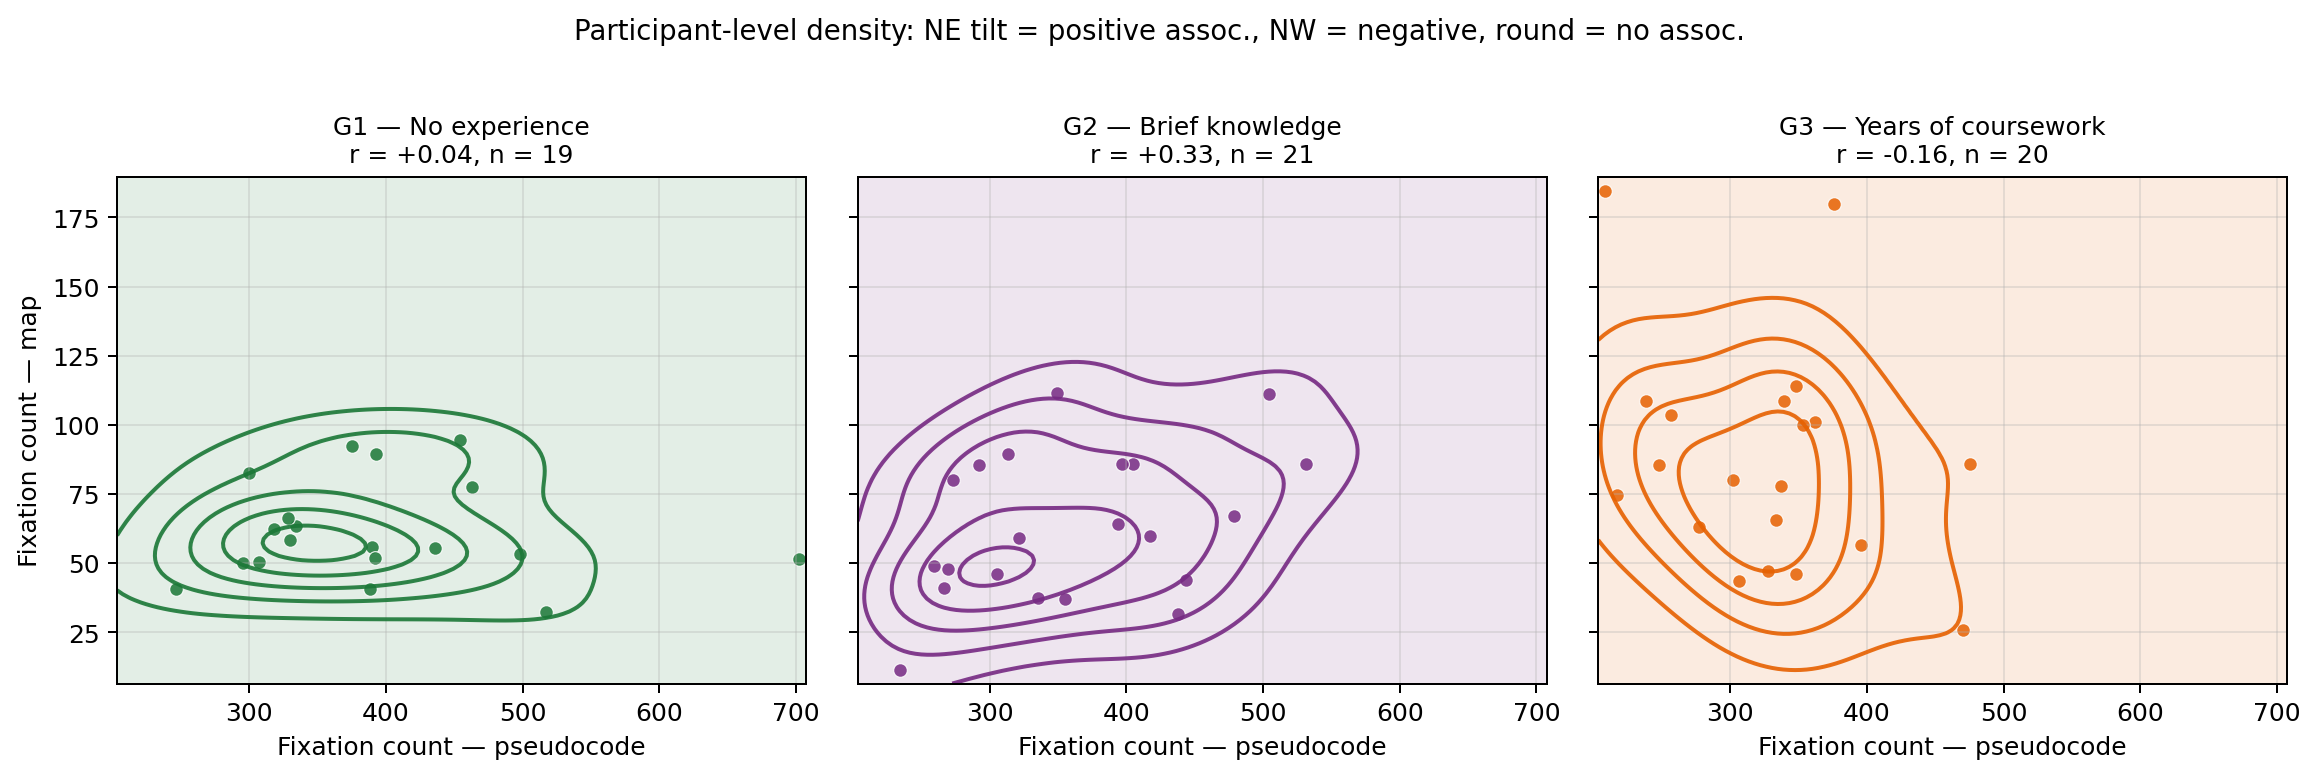
\includegraphics[width=\columnwidth, alt={KDE contour plots for G1, G2, and G3. G2 ellipse tilts northeast indicating positive correlation. G3 ellipse tilts northwest indicating negative correlation. G1 is roughly circular.}]{fig3_kde_contours}
  \caption{%
    Kernel density contours for each group. Northeast orientation (G2)
    indicates positive association; northwest orientation (G3) indicates
    negative association; circular shape (G1) indicates no relationship.
  }
  \label{fig:kde}
\end{figure}

% ^^
The monotonic strengthening of negative TFD correlation matches what ERE
predicts for multi-representation learning. Novices attend the two panels
independently, neither coordinating nor trading off between them.
Intermediate viewers begin to trade dwell time between the panels.
Experienced viewers trade off most strongly. Under this pattern, dwell on
the two panels becomes increasingly a zero-sum allocation as schema
develops; the coordination CTML predicts from a dual-channel format does
not appear in any group's dwell data.
% ^^

\subsection{Attentional Coupling}

Our study suggests a monotonic increase in attentional coupling across
expertise levels. Mean absolute Spearman $r$ across all metric pairs was 0.294
for G1, 0.330 for G2, and 0.369 for G3. Those participants less experienced
with the subject matter were more likely to show independent metrics. The
ratio-to-scanner\_index pair, for example, goes from $r$=$-$0.04 in G1 to
$r$=$-$0.67 in G3. Studies that pool expertise levels mix participants whose
attention is organized by different mechanisms, and the resulting averages do
not reflect any single group's behavior.


\section{Discussion}

\subsection{Mechanism}

% ^^
The monotonic strengthening of negative TFD correlation in
\cref{sec:reversal} follows from the interaction of CLT and ERE across the
three groups.

G1 viewers have no prior schema for BFS or DFS. Working memory is occupied
by a novel algorithm and a novel visual format at the same time. With no
schema available to link the two panels, dwell time on each is largely
independent of dwell time on the other.

G2 viewers have a partial schema. Some steps of the algorithm are
predictable from either panel alone; others still require both. Dwell on
the pseudocode panel begins to offset dwell on the map as the predictable
steps become easier to anticipate. The directional positive trend in
fixation count suggests that confirmatory visits between panels remain
frequent even as dwell times begin to trade off.

G3 viewers have internalized the algorithm. Either panel carries enough
information to anticipate the next step, so time spent on one panel is
time that no longer needs to be spent on the other. Dwell on the two
panels becomes strongly negatively correlated.

The inverted-U in pseudocode-to-map ratio (\cref{sec:inverted}) and the
monotonic substitution in dwell time (\cref{sec:reversal}) reflect the
same mechanism at two scales: overall attention allocation and
moment-to-moment dwell trade-offs.
% ^^

\subsection{Design Implications}

% ^^
While fixations and visits do not inherently equate to active engagement
with the material, the substitution gradient suggests each expertise group
uses the split-panel design differently. For G1, dwell on the two panels
is independent; scaffolding such as line highlights, annotations, or
staged display may be needed to promote coordination before presenting
both panels at once. G2 partially substitutes between the panels while
still engaging both, which is the profile the split-panel format fits
best. For G3, the pseudocode panel functions as a quick verification
check rather than a primary source of information; either representation
alone would likely suffice.
% ^^

Our findings also suggest that the algorithm being visualized matters more for
novices than for experienced viewers. Attention metrics evaluated without
stratifying by expertise level will produce averages that do not describe any
group accurately.

\subsection{Limitations}

% ^^
The Fisher z-test battery ran around 105 comparisons; at $p$<.05, about
five false positives are expected by chance. The primary TFD-based finding
in \cref{sec:reversal} reaches $p$=.04 for the G1 vs G3 contrast, which
survives that threshold even under modest correction. The secondary
fixation-count sign reversal is directional rather than inferential at the
participant level.
% ^^
Expertise groups were not randomized; observed differences may correlate
with general ability or motivation rather than programming knowledge
specifically. All visualizations used the Metal style, and generalizability
to other animation designs is not established. Group sizes of roughly 19
to 21 participants per group limit power to detect small correlation
differences.

\subsection{Conclusion}

% ^^
Pseudocode-panel and geospatial-map dwell times trade off more strongly as
programming expertise grows. Novices attend the two panels independently;
intermediate and experienced viewers increasingly substitute one for the
other. Designers targeting a single expertise level should not assume that
a layout validated on one group will generalize to the others, and studies
that pool across levels may obscure this substitution gradient.
% ^^


\section*{Supplemental Materials}

Data and analysis notebooks are available at [URL].


\acknowledgments{%
  [ACKNOWLEDGMENTS]
}


\bibliographystyle{abbrv-doi-hyperref}
\bibliography{paper}


\end{document}
